%%%%%%%%%%%%%%%%%%%%%%%%%%%%%%%%%%%%%%%%%
% a0poster Portrait Poster 
% LaTeX Template
% with University Copenhagen logo
% Version 1.0 (22/06/13)
%
% Based on:
% The a0poster class was created by:
% Gerlinde Kettl and Matthias Weiser (tex@kettl.de)
% 
% This template has been downloaded from:
% http://www.LaTeXTemplates.com
%
%%%%%%%%%%%%%%%%%%%%%%%%%%%%%%%%%%%%%%%%%

%----------------------------------------------------------------------------------------
%	PACKAGES AND OTHER DOCUMENT CONFIGURATIONS
%----------------------------------------------------------------------------------------

\documentclass[a0,portrait]{a0poster}
\usepackage[utf8]{inputenc}

\usepackage{multicol} % This is so we can have multiple columns of text side-by-side
\columnsep=100pt % This is the amount of white space between the columns in the poster
\columnseprule=3pt % This is the thickness of the black line between the columns in the poster

\usepackage[svgnames]{xcolor} % Specify colors by their 'svgnames', for a full list of all colors available see here: http://www.latextemplates.com/svgnames-colors

\usepackage{times} % Use the times font
%\usepackage{palatino} % Uncomment to use the Palatino font

\usepackage{graphicx} % Required for including images
\graphicspath{{figures/}} % Location of the graphics files
\usepackage{booktabs} % Top and bottom rules for table
\usepackage[font=small,labelfont=bf]{caption} % Required for specifying captions to tables and figures
\usepackage{amsfonts, amsmath, amsthm, amssymb} % For math fonts, symbols and environments
\usepackage{wrapfig} % Allows wrapping text around tables and figures
\definecolor{ku}{RGB}{144,26,30}
\definecolor{ku-yellow}{RGB}{255,249,25}

 \usepackage{eso-pic}
               \newcommand\BackgroundIm{
               }

\begin{document}
%----------------------------------------------------------------------------------------
%	POSTER HEADER 
%----------------------------------------------------------------------------------------

% The header is divided into two boxes:
% The first is 75% wide and houses the title, subtitle, names, university/organization and contact information
% The second is 25% wide and houses a logo for your university/organization or a photo of you
% The widths of these boxes can be easily edited to accommodate your content as you see fit

\begin{minipage}[t]{0.60\linewidth}
\vspace{1cm} % Reduced vertical space
\Huge \color{ku} \textbf{Enhancing Art Classification: A Comparative Study of CNN, Transfer Learning, and SVM Models} \color{Black}\\[0.5cm]
\huge\textit{A Comprehensive Approach to Identifying Art Styles}\\[1cm]
\Large \textbf{Aditya Prakash (22201796), Shreya Grover (22200383)}\\[0.5cm]
\Large School of Mathematics and Statistics, University College Dublin

\end{minipage}
%
\begin{minipage}[t]{0.40\linewidth}
\vspace{1cm} % Reduced vertical space
\flushright
\color{DarkSlateGray}
\Large \textbf{Contact Information:}\\
Email: \texttt{aditya.prakash@ucdconnect.ie}\\% Email address
\texttt{shreya.grover@ucdconnect.ie}
\end{minipage}

\vspace{1cm} % A bit of extra whitespace between the header and poster content

%----------------------------------------------------------------------------------------

\begin{multicols}{2} % This is how many columns your poster will be broken into, a portrait poster is generally split into 2 columns

%----------------------------------------------------------------------------------------
%	INTRODUCTION
%----------------------------------------------------------------------------------------

\color{SaddleBrown} % SaddleBrown color for the introduction

\section*{Introduction}

Art classification and authentication have been subjects of increasing interest in both the art and scientific communities. Techniques such as automated analysis of drawings at the stroke level have been applied for attribution and authentication \cite{elgammal2017picasso}. Additionally, machine learning has been utilized for the identification of art paintings \cite{Blessing2010UsingML}.

\begin{center}
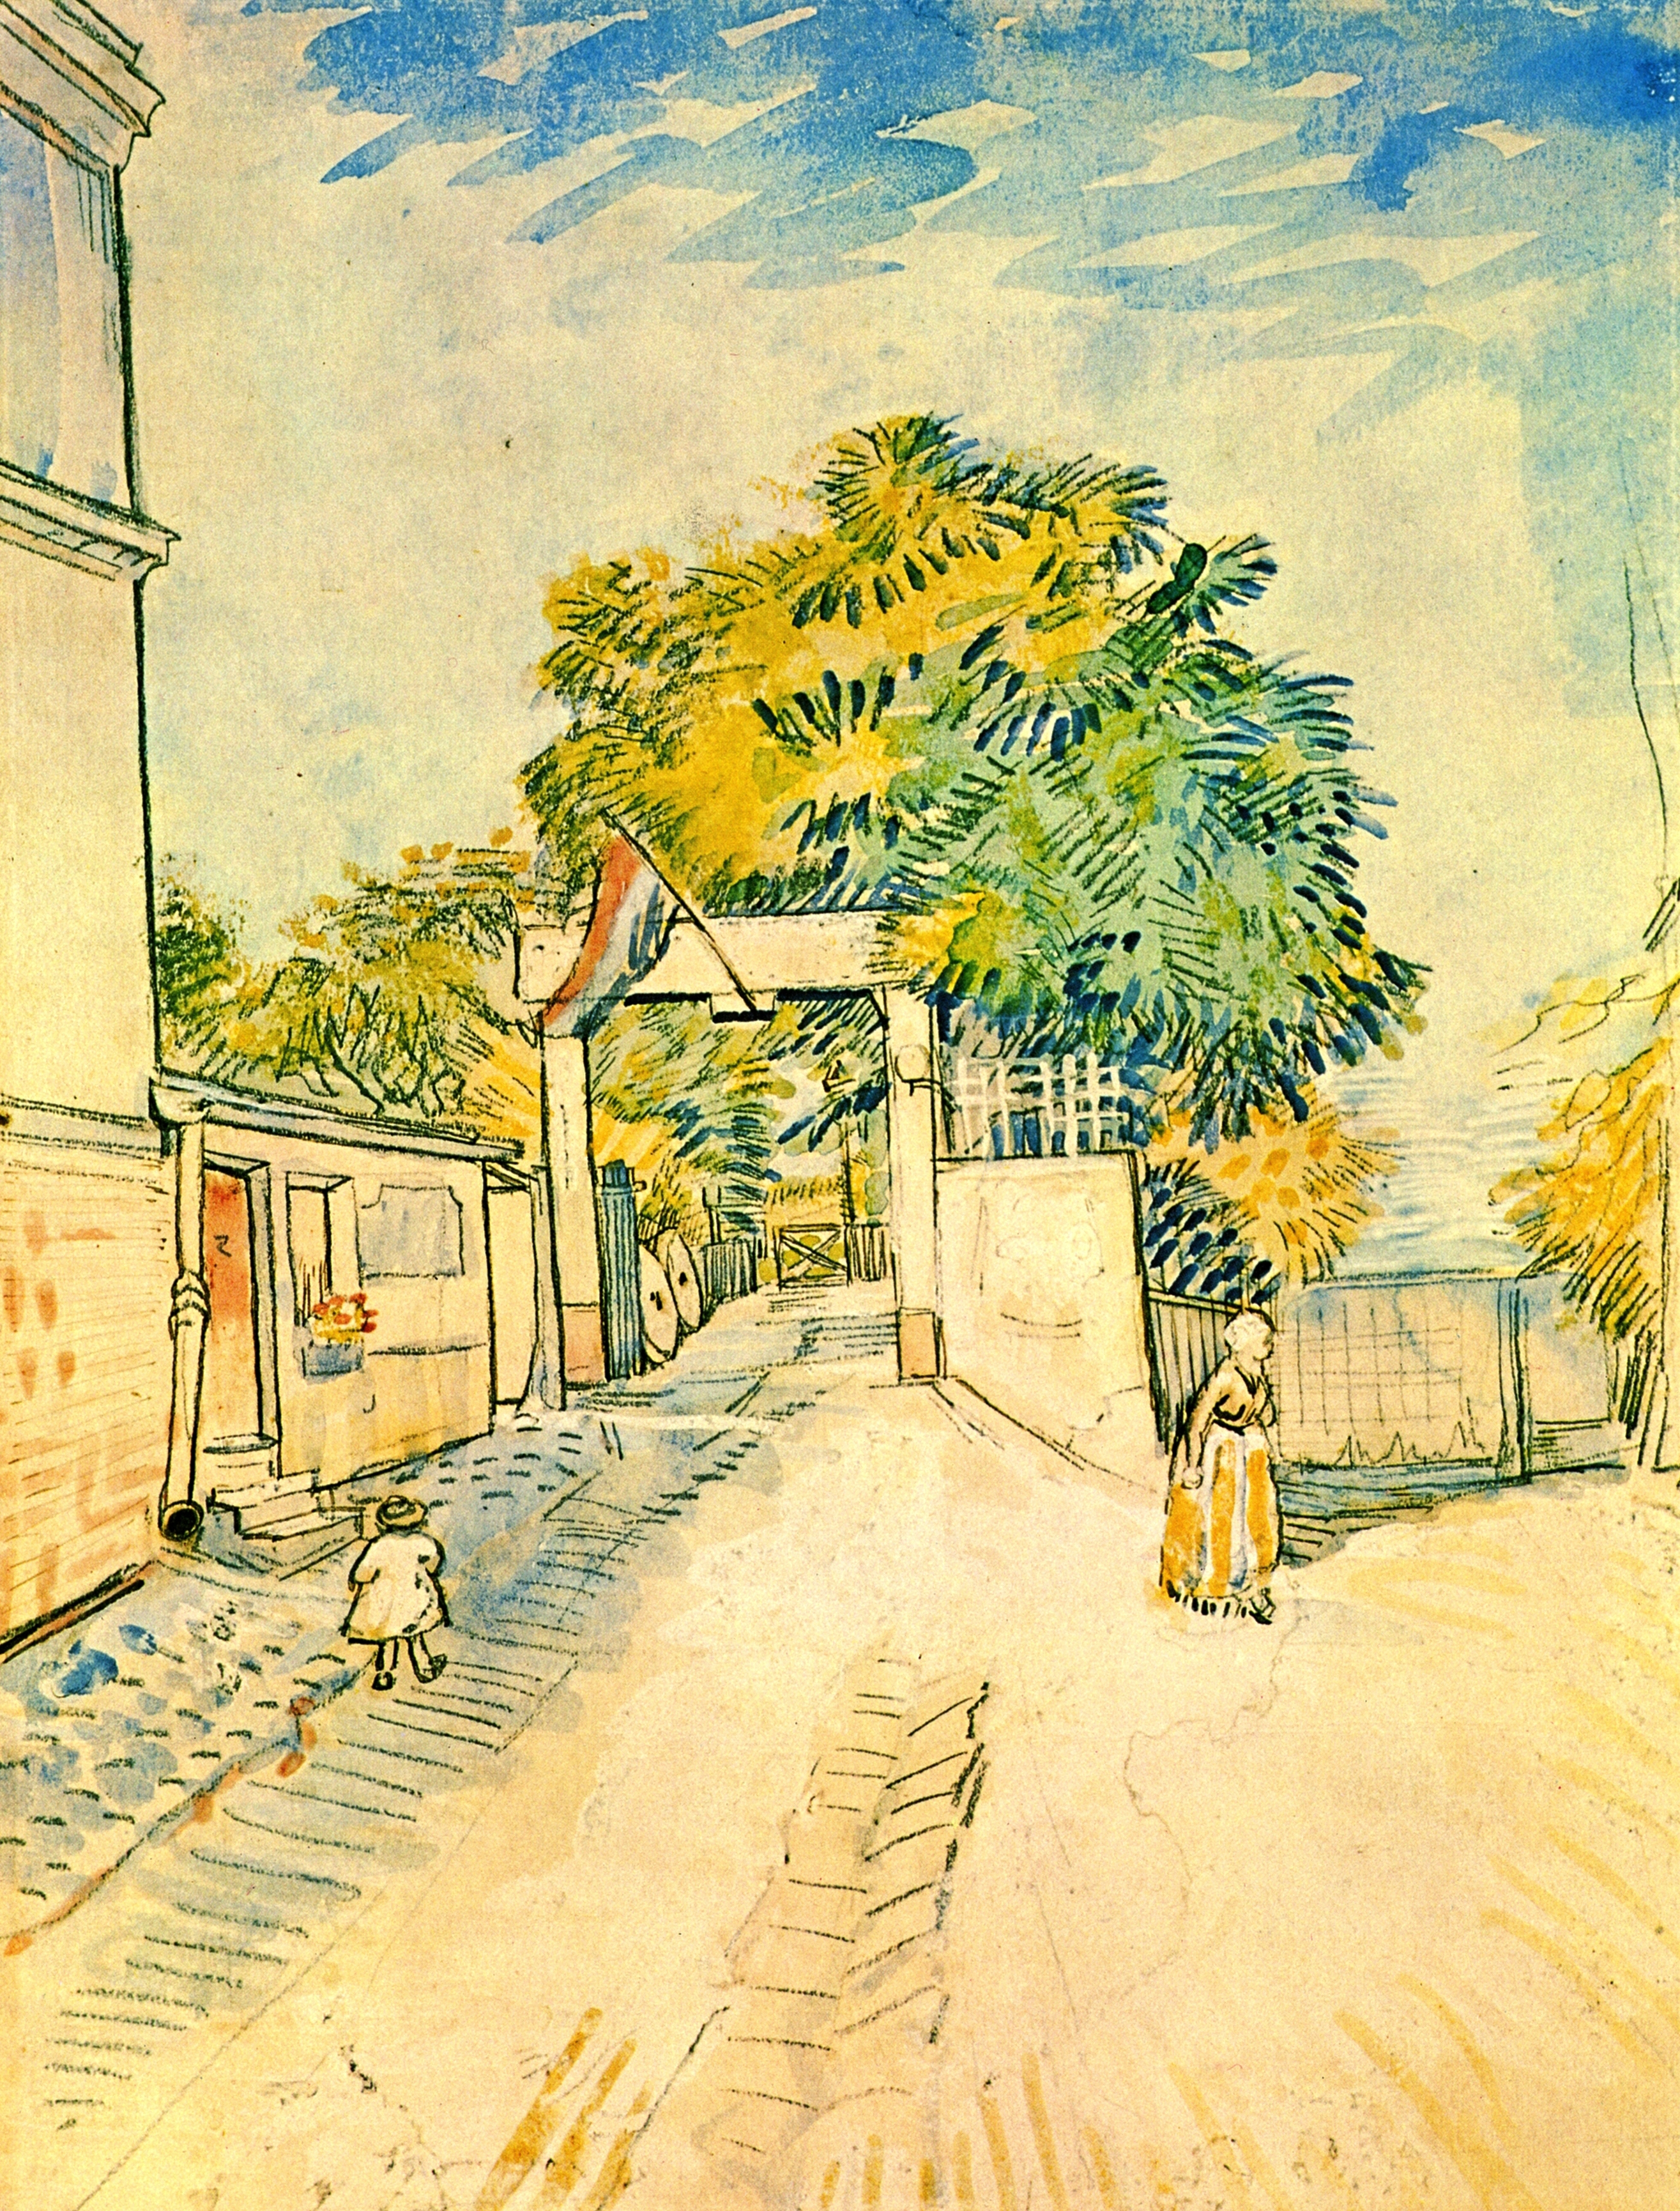
\includegraphics[height=0.20\linewidth]{figures/75309.jpg} % Scaled to match the height of 64331.jpg
\includegraphics[height=0.20\linewidth]{figures/64331.jpg} % No scaling needed
\includegraphics[height=0.20\linewidth]{figures/40524.jpg} % Scaled to match the height of 64331.jpg
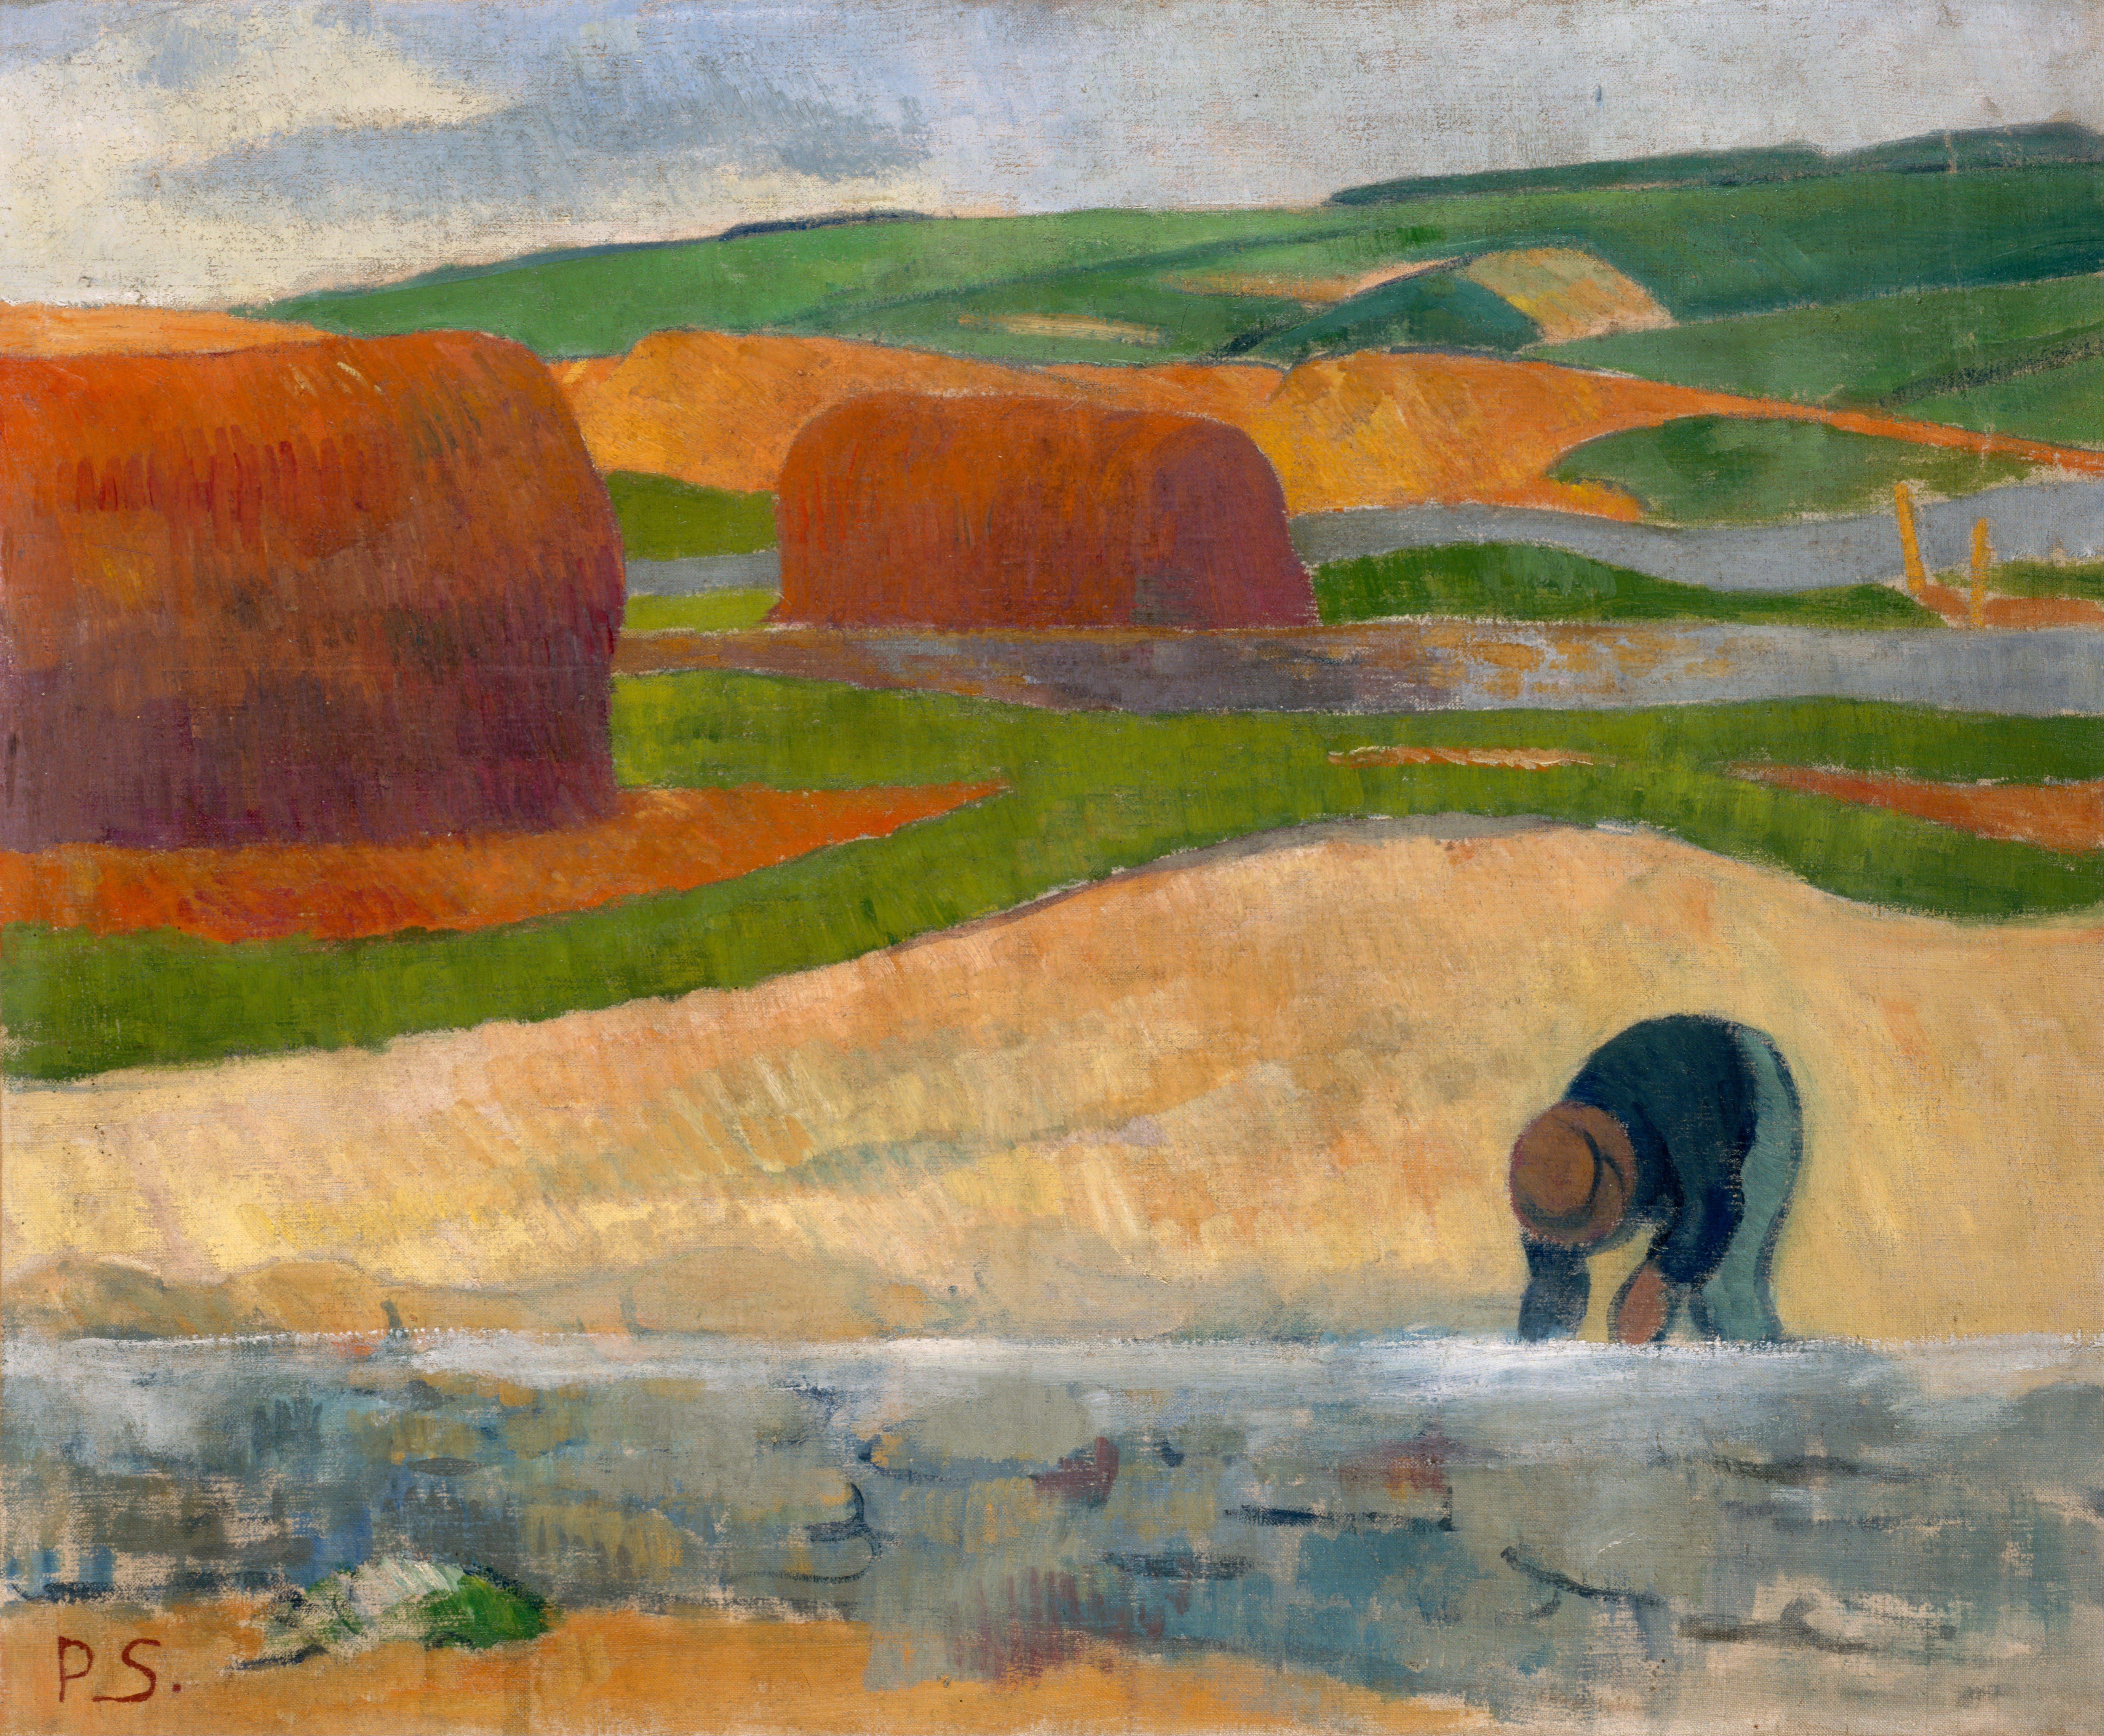
\includegraphics[height=0.20\linewidth, keepaspectratio]{figures/32996.jpg} % Scaled to be the same height, but width is proportionate
\captionof{figure}{\color{Green} Some of the paintings used in the dataset. Works by Van Gogh, Matisse, Toyokuni, and Aivazovsky.}
\end{center}

% ...

%----------------------------------------------------------------------------------------
%	DATASET DESCRIPTION
%----------------------------------------------------------------------------------------

\section*{Dataset Description}

The dataset primarily sourced from WikiArt.org encompasses a total of 2,319 different artists and 43 unique painting genres. For practical classification, a threshold of 500 paintings per artist was set to filter the dataset, resulting in a balanced selection that includes 12 different artists and 30 unique painting genres.

\begin{itemize}
\item \textbf{Total Artists:} 12
\item \textbf{Total Genres:} 30
\item \textbf{Artists Included:} Ivan Aivazovsky, Gustave Dore, Rembrandt, Pierre-Auguste Renoir, Albrecht Durer, Ivan Shishkin, Giovanni Battista Piranesi, John Singer Sargent, Zdislav Beksinski, Ilya Repin, Pablo Picasso, Marc Chagall
\end{itemize}

This approach ensures a robust dataset for classification by excluding artists with insufficient samples and retaining those with substantial numbers. The images in the dataset are utilized exclusively for data mining, adhering to fair use principles, and are assumed to be protected by copyright.

%----------------------------------------------------------------------------------------
%	OBJECTIVES
%----------------------------------------------------------------------------------------

\color{DarkSlateGray} % DarkSlateGray color for the rest of the content

\section*{Main Objectives}
\begin{enumerate}
\item Develop a custom CNN for art classification.
\item Utilize transfer learning with ResNet50 for enhanced performance.
\item Implement a multi-class SVM using various feature extraction methods.
\item Analyze and compare the performance of the three models.
\end{enumerate}

%----------------------------------------------------------------------------------------
%	MATERIALS AND METHODS
%----------------------------------------------------------------------------------------

\section*{Materials and Methods}

A tailor-made Convolutional Neural Network (CNN) is developed for art classification, comprising multiple convolutional layers, activation functions, and a fully connected layer. Leveraging the pre-trained ResNet50 model, fine-tuning is performed to adapt to the specific art classification task. Additionally, a Support Vector Machine (SVM) classifier is implemented, utilizing various feature extraction techniques such as SIFT, HOG, ORB, and Gabor filters. The dataset is preprocessed to include only artists with at least 500 paintings and the artist names are encoded. The data is then split into training and validation sets for model training.

%------------------------------------------------

\subsection*{Mathematical Formulation of Models}

\subsection*{Custom CNN}
A Convolutional Neural Network (CNN) consists of convolutional layers, activation functions, pooling layers, and fully connected layers.

\begin{itemize}
\item \textbf{Convolutional Layer}: Applies a convolution operation to the input, passing the result to the next layer. Mathematically, the convolution is expressed as:
  \[
f * g(x, y) = \sum_m \sum_n f(m, n) \cdot g(x \cdot s - m + p, y \cdot s - n + p)
\]
\item \textbf{Activation Function}: Introduces non-linear properties to the system. Commonly used is the ReLU (Rectified Linear Unit) function:
  \[
f(x) = \max(0, x)
\]

\item \textbf{Pooling Layer}: Reduces the spatial size of the representation, commonly using max pooling:
  \[
f(x, y) = \max_{(m, n) \in W} g(x + m, y + n)
\]
  where \( W \) is the window size.
\item \textbf{Fully Connected Layer}: Connects every neuron in one layer to every neuron in the next layer, typically used in the final classification step.
\end{itemize}

\subsection*{Transfer Learning using ResNet50}
ResNet (Residual Network) leverages residual connections or "skip connections" that bypass one or more layers. The residual block can be expressed as:
\[
\mathbf{F}(\mathbf{x}) = \mathbf{H}(\mathbf{x}) - \mathbf{x}
\]
where \( \mathbf{F}(\mathbf{x}) \) is the residual mapping to be learned, and \( \mathbf{H}(\mathbf{x}) \) is the desired mapping.

Transfer learning involves utilizing a pre-trained model (e.g., trained on ImageNet) and fine-tuning it for a specific task.

\subsection*{Multi-Class SVM with SIFT, HOG, ORB, and Gabor}
A Support Vector Machine (SVM) finds the hyperplane that best separates the classes.

\begin{itemize}
\item \textbf{Hyperplane Equation}:
  \[
  \mathbf{w} \cdot \mathbf{x} + b = 0
  \]
  where \( \mathbf{w} \) is the weight vector, \( \mathbf{x} \) is the input vector, and \( b \) is the bias.
\item \textbf{Feature Extraction}:
  \begin{itemize}
  \item \textbf{SIFT} (Scale-Invariant Feature Transform): Detects and describes local features.
  \item \textbf{HOG} (Histogram of Oriented Gradients): Captures the gradient orientation in localized portions.
  \item \textbf{ORB} (Oriented FAST and Rotated BRIEF): A fast binary descriptor.
  \item \textbf{Gabor Filters}: Used for texture representation and discrimination.
  \end{itemize}
\end{itemize}
%----------------------------------------------------------------------------------------
%	RESULTS 
%----------------------------------------------------------------------------------------

\section*{Results}

The test results of the experiments with the custom CNN, ResNet50, and SVM models are summarized in the table below:

\begin{center}
\begin{tabular}{l c c}
\toprule
\textbf{Model} & \textbf{Test Loss} & \textbf{Test Accuracy} \\
\midrule
CNN & 1.2615 & 59.70\% \\
ResNet & 0.9001 & 72.37\% \\
SVM & N/A & 55.67\% \\ 
\bottomrule
\end{tabular}
\captionof{table}{Comparison of test loss and accuracy for the custom CNN, ResNet50, and SVM models.}
\end{center}

\begin{center}\vspace{1cm}
\includegraphics[width=0.6\linewidth]{figures/cnn_output.png}
\includegraphics[width=0.6\linewidth]{figures/resnet_output.png}
\captionof{figure}{\color{Green} The first two images show the Training and Validation Losses and Accuracies for the custom CNN. The latter two images show the Training and Validation Losses and Accuracies for the ResNet model.}
\end{center}\vspace{1cm}

%----------------------------------------------------------------------------------------
%	CONCLUSIONS
%----------------------------------------------------------------------------------------

\color{SaddleBrown} % SaddleBrown color for the conclusions to make them stand out

\section*{Conclusions}

\begin{itemize}
\item The study explored the task of art classification through three different approaches: a custom CNN, ResNet50, and a multi-class SVM. Each method provided unique insights into the complexities of classifying artworks based on artists.
\item ResNet50, leveraging transfer learning, stood out as the top-performing model, highlighting the effectiveness of pretrained deep learning models in handling complex visual patterns.
\item The custom CNN offered a balance between model complexity and performance, showcasing the potential of tailored convolutional networks in art classification.
\item The multi-class SVM with multiple feature extractions demonstrated the versatility of traditional machine learning techniques when combined with various image feature extractions.
\item The comparative analysis not only underscores the strengths and weaknesses of each approach but also opens avenues for future research. The exploration of Generative Adversarial Networks (GANs) for art forgery detection is particularly promising, which can further broaden the application of machine learning in art authentication and analysis.
\end{itemize}


\color{DarkSlateGray} % Set the color back to DarkSlateGray for the rest of the content

%----------------------------------------------------------------------------------------
%	FURTHER RESEARCH
%----------------------------------------------------------------------------------------

\section*{Further Research}

The future research direction includes exploring the application of Generative Adversarial Networks (GANs) for art forgery authentication. GANs, composed of a generator and a discriminator, could be employed to recognize nuanced characteristics of an artist's style, such as brush strokes and colour palettes. By training on authentic art pieces, the network might discern genuine works from forgeries. Though promising, this approach presents challenges, such as the potential misuse of the GAN to create convincing fakes. Integrating GANs with existing models like CNN, ResNet50, and SVM could result in a comprehensive and more robust art authentication system.

 %----------------------------------------------------------------------------------------
%	REFERENCES
%----------------------------------------------------------------------------------------

\nocite{*} % Print all references regardless of whether they were cited in the poster or not
\bibliographystyle{plain} % Plain referencing style
\bibliography{sample} % Use the example bibliography file sample.bib

\end{multicols}
\end{document}